% AdaptiveRAG Architecture Figure (standalone TikZ)
% Compile with: pdflatex architecture.tex
\documentclass[border=5pt]{standalone}
\usepackage{tikz}
\usetikzlibrary{shapes.geometric, arrows.meta, positioning, fit}

\begin{document}
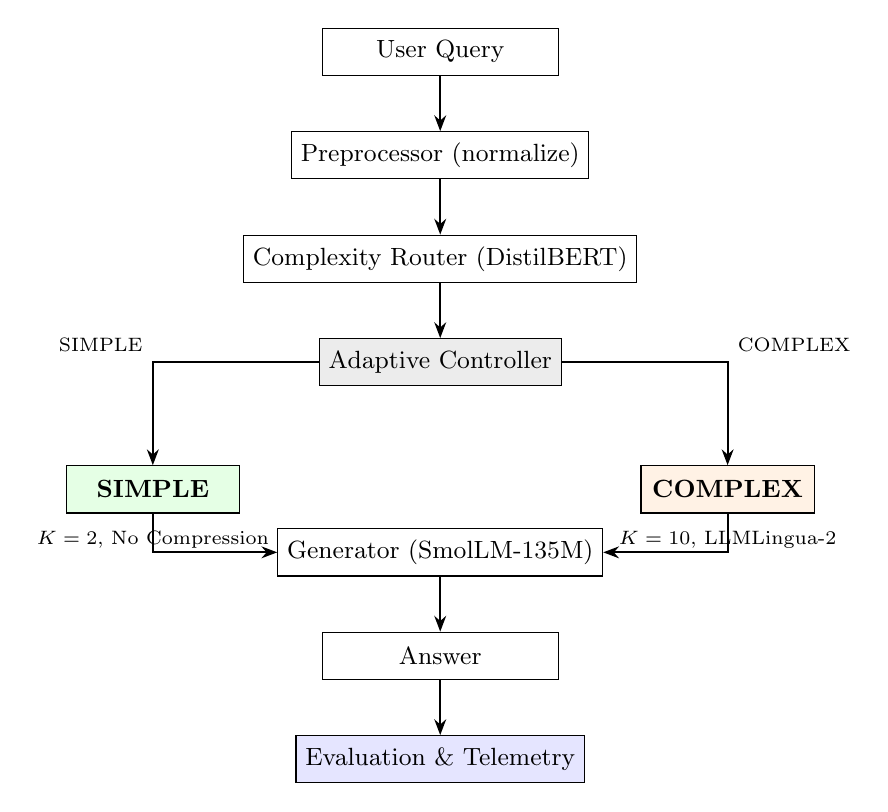
\begin{tikzpicture}[
    node distance=0.7cm,
    block/.style={rectangle, draw, text centered, minimum width=3.0cm, minimum height=0.6cm, font=\small},
    arrow/.style={-{Stealth[length=2mm]}, thick},
    label/.style={font=\scriptsize}
]

\node[block] (query) {User Query};
\node[block, below=of query] (preproc) {Preprocessor (normalize)};
\node[block, below=of preproc] (router) {Complexity Router (DistilBERT)};
\node[block, below=of router, fill=gray!15] (controller) {Adaptive Controller};

\node[block, below left=1.0cm and 1.0cm of controller, minimum width=2.2cm, fill=green!10] (simple) {\textbf{SIMPLE}};
\node[block, below right=1.0cm and 1.0cm of controller, minimum width=2.2cm, fill=orange!10] (complex) {\textbf{COMPLEX}};

\node[label, below=0.1cm of simple] (slabel) {$K=2$, No Compression};
\node[label, below=0.1cm of complex] (clabel) {$K=10$, LLMLingua-2};

\node[block, below=1.8cm of controller] (gen) {Generator (SmolLM-135M)};
\node[block, below=of gen] (answer) {Answer};
\node[block, below=of answer, fill=blue!10] (eval) {Evaluation \& Telemetry};

\draw[arrow] (query) -- (preproc);
\draw[arrow] (preproc) -- (router);
\draw[arrow] (router) -- (controller);
\draw[arrow] (controller) -| node[above left, font=\scriptsize]{SIMPLE} (simple);
\draw[arrow] (controller) -| node[above right, font=\scriptsize]{COMPLEX} (complex);
\draw[arrow] (simple) |- (gen);
\draw[arrow] (complex) |- (gen);
\draw[arrow] (gen) -- (answer);
\draw[arrow] (answer) -- (eval);

\end{tikzpicture}
\end{document}
